\documentclass{article}
\usepackage{minted}
\usepackage{listings}
\usepackage{amsmath}
\usepackage{amssymb}
\usepackage{hyperref}
\usepackage{tikz}
\usetikzlibrary{shapes.geometric}
\usetikzlibrary{decorations.pathreplacing,calligraphy}
\usetikzlibrary{positioning}

\newcommand{\pkg}[1]{\href{https://ctan.org/pkg/#1}{\texttt{#1}}}
\newcommand{\texcmd}[1]{\texttt{\textbackslash#1}}

\begin{document}

\section{Math Formula}
 \label{sec:math} \par Current \LaTeX parser will convert inline math formula
(e.g. Einstein 's
\begin{math}
  E=mc^2
\end{math}
 ) into the \texttt{math} environment, and display line-spreading math formula
(as the one shown below) into the \texttt{equation} environment. These are
defined in \pkg{amsmath} package, and are widely used in scientific documents.
\begin{displaymath}
  E=mc^2.
\end{displaymath}
 \par Below is a numbered \texttt{equation} environment, which is also
supported by our parser.
\begin{equation}
  E=mc^2
\end{equation}
 . For very long formulas like
\begin{math}
  \Biggl\lvert\biggl\lvert\Bigl\lvert\bigl\lvert\lvert x \rvert\bigr\rvert\Bigr
  \rvert\biggr\rvert\Biggr\rvert
\end{math}
 , the parser will automatically add line-breaks for readability. \par Note
that the plainTex \$\$ line-spreading math mode is not supported and results in
error during parsing.

\section{Listings}
 \label{sec:listings} \par Our \LaTeX parser will also handle code listings,
which are often used in scientific documents to present algorithms, code
snippets, or command-line instructions. The parser recognizes environments such
as \texttt{minted} (from \pkg{minted} package) and \texttt{lstlisting} (from
\pkg{listings} package) as code environments, and copies-pasts the contained
code \textbf{as-is}. Even though listings embedded in the \LaTeX document can
be handled \textit{most of the time}, it is recommended to put them in separate
files and use \texcmd{inputminted} or \texcmd{lstinputlisting} to embed them in
the document. \par Till the next section, the provided listings are for testing
purposes.
\begin{lstlisting}[language=Python]
# this snippet checks that auto linebreak is disabled in code environments.
class Formatter():
    __slots__ = ['writer']
    def __init__(self, buf: io.TextIOBase | io.TextIOWrapper,
                 indent_size: int = 2,
                 linebreak: str = '\n',
                 line_length: int = 80):
        config: PrettyWriter.Config = PrettyWriter.Config(indent_size, linebreak, line_length)
        self.writer = PrettyWriter(buf, config)
\end{lstlisting}
 \par The folloing snippet checks handling of backslash in code environments,
which is often used in C/C++ for line continuation.
\begin{minted}{c}
uint32_t safe_rem(uint32_t a, uint32_t b) {
  if (b == 0) {
    errno = EINVAL;
    return 0;
  }
  return a % b; // should not be parsed as LaTex comment.     
}

#define unlikely __builtin_expect(!!(cond), 0)
#define assert(cond)                                                           \
  do {                                                                         \
    if (unlikely(cond)) {                                                      \
      __assert_fail(#cond, __FILE__, __LINE__, __func__);                      \
    }                                                                          \
  } while (0)
\end{minted}

\section{Figures and Tables}
 \label{sec:figtab} \par The parser also supports figures (e.g. Figure~
\ref{fig:venn}) and tables (e.g Table~\ref{tab:pub}), which are commonly used
to present visual data and structured information in scientific documents. The
parser will format the table in a quite simple manner, although more complex
ones (e.g. aligning columns and \& operator) may be added in the future.
\begin{figure*}[ht]
  \centering 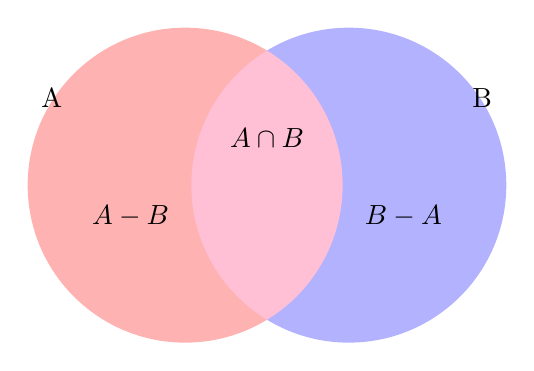
\begin{tikzpicture}
    \begin{scope}[blend group = soft light]
      \fill[red!30!white] (210:1.2) circle (2); \fill[blue!30!white] (330:1.2)
      circle (2);
    \end{scope} \node (n0) at ( 210:2) {\begin{math}
      A-B
    \end{math}}; \node (n1) at ( 330:2) {\begin{math}
      B - A
    \end{math}}; \node {\begin{math}
      A\cap B
    \end{math}}; \node (a0) [above=of n0, xshift=-1cm] {A}; \node (a1) [
    above=of n1, xshift=1cm] {B};
  \end{tikzpicture} \caption{Binary operators on sets {A} and {B}. \\
  {\small The figure caption is usually placed \textbf{below} the figure.}
  } \label{fig:venn}
\end{figure*}
\begin{table}[ht]
  \centering \caption{Number of publications by year (from forged data).}
  \label{tab:pub} \begin{tabular}{lcc}
  \hline
  Year & Number of Publications \\
  \hline
  2020 & 100 \\
  2021 & 150 \\
  2022 & 200 \\
  2023 & 250 \\
  \hline
  \end{tabular}
\end{table}

\section{Structuring the Document}
 \label{sec:struct} \par A document's element types include \texcmd{chapter}
(optional, usually for the book \texcmd{documentclass}), \texcmd{section},
\texcmd{subsection}, \texcmd{subsubsection}, and \texcmd{paragraph}. \par
Structuring chapters and sections are done in function
\texttt{struct\_sections} ; paragraph structure are parsed in method
\texttt{split\_by\_paragraphs} in class \texttt{EnvironNode}. Paragraph
splitting is done by finding the \texcmd{par}, \texcmd{paragraph} commands and
empty lines.

\section{Applications of Our Parser}
 \label{sec:apply}
\paragraph*{Document Formatting} This document is neatly formatted by our
formatter. Formatting options include (maximum) line length, line break (can be
LF or CRLF), and indent size.

\end{document}


